\documentclass[xcolor=svgnames]{beamer}
\usetheme[
    %%% options passed to the outer theme
    %    hidetitle,           % hide the (short) title in the sidebar
    %    hideauthor,          % hide the (short) author in the sidebar
    %    hideinstitute,       % hide the (short) institute in the bottom of the sidebar
    %    shownavsym,          % show the navigation symbols
         width=1.5cm,         % width of the sidebar (default is 2 cm)
    %    hideothersubsections,% hide all subsections but the subsections in the current section
    %    hideallsubsections,  % hide all subsections
         left                 % right of left position of sidebar (default is right)
    %%% options passed to the color theme
        lightheaderbg         % use a light header background
  ]{AAUsidebar}
\setbeameroption{show notes}

% #### graphics and schemes
\usepackage{graphicx}
\graphicspath{{img/}}
\usepackage{tikz}
\usetikzlibrary{                          % TikZ libraries
                scopes,                   % .
                shapes,                   % .
                arrows,                   % .
                through,                  % .
                calc,                     % .
                intersections,            % .
                spy,                      % .
                matrix,                   % .
                chains,                   % .
                mindmap,                  % .
                trees,                    % .
                decorations.pathreplacing,% .
                decorations.pathmorphing, % .
                decorations.markings}     % .

\usepackage{pgfplots}                     % TikZ plots
\usepackage{pgfplotstable}                % TikZ tables from CSV
\pgfplotsset{compat=1.3}                  % activates \xilabel shift` for pgfplots
\usepackage{array}
\usepackage{listings}
\usepackage{times}
\usepackage{amsmath}
\usepackage{verbatim}
\usepackage{ccicons}
\usepackage{tcolorbox}
\usepackage{chronosys}
\usepackage{listings}                     % code
\usepackage{adjustbox}                    % code
\usepackage{attrib}

% #### colors
\usepackage{xcolor}                       % common color names
\usepackage{colortbl}                     % common color names

% #### layouts
\usepackage{multicol}
\usepackage[textfont=footnotesize,bf]{caption}
\usepackage{subfig}

% #### fonts
\usepackage[utf8]{inputenc}
\usepackage[english]{babel}
\usepackage[T1]{fontenc}
\usepackage{cmbright}
\usepackage{soul} %slanted text
\usepackage{hyperref}
\urlstyle{same}
\hypersetup{pdfauthor={Francesco de Virgilio},pdftitle={Handling GRIB files: when NOT to use GIS to manage geographic data}}

% #### tables
\usepackage{booktabs}			          % migliora la qualità delle tabelle
\usepackage{tabularx}			          % colonne a spaziatura fissa delle tabelle
\newcommand{\otoprule}                    % better top rule horizontal line
    {\midrule[\heavyrulewidth]}           % .


\begin{document}

\usebackgroundtemplate{%
    
\includegraphics[width=\paperwidth,height=\paperheight]{img/back_first}}

    \begin{frame}[plain,noframenumbering]
        \begin{center}
            \color{white}
            \LARGE{Handling weather GRIB files}\\
            \normalsize{When \textit{not} to use GIS to manage geographic data}\\
            \vspace{40pt}
            Francesco de Virgilio\\
            \vspace{8pt}
            \scriptsize{Pole Star Space Applications}\\
            \scriptsize{London, 27 Jan 2015}
        \end{center}
    \end{frame}

\usebackgroundtemplate{%
    
\includegraphics[width=\paperwidth,height=\paperheight]{img/back_normal}}

\section{GIS}

    \begin{frame}{Lower your expectations}
        \pause
        This talk will:
        \begin{itemize}
            \item help you to understand the WeatherAPI
            \pause
            \item mess up your ideas about GRIB files
        \end{itemize}
        \pause
        \vspace{0.05\textwidth}
        This talk \textbf{will not}:
        \begin{itemize}
            \item talk about GIS software (surprise!)
            \pause
            \item help you to discover your true self
            \pause
            \item save dolphins and kittens
        \end{itemize}
    \end{frame}

    \begin{frame}{GIS in Pole Star}
        \begin{center}
            \color{black}
            \begin{block}{Geographic Information System}
                Is a computer system designed to capture, store, manipulate, analyze, manage, and present all types of spatial or geographical data.
            \end{block}
        \end{center}
        \vspace{0.05\textheight}
        \only<2->{Extensions to well-known software}
        \begin{columns}[c]
            \column{.5\textwidth}
                \begin{itemize}
                    \item<2-> Django
                    \item<3-> PostgreSQL
                \end{itemize}
            \column{.5\textwidth}
                \begin{itemize}
                    \item<2-> geoDjango
                    \item<3-> PostGIS
                \end{itemize}
        \end{columns}
    \end{frame}

   \subsection{GIS balancing}

        \begin{frame}{GIS is about balance}
            Pros:
            \begin{itemize}
                \item functions to ease some calculations
                \item quicker data retrieval and analysis
                \item good integration with OO languages (Python/geoDjango)
            \end{itemize}
            \pause
            \vspace{0.05\textwidth}
            Cons:
            \begin{itemize}
                \item avg geospatial package is less well-maintained than other packages (pip, CentOS)
                \pause
                \item lack of support for some well-known formats (PostGIS 1.5 and GRIB)
                \pause
                \item \textbf{GIS is only effective on properly-structured data}
            \end{itemize}
        \end{frame}

\section{Weather}

    \subsection{Objective}

        \begin{frame}{Issue}
            \begin{block}{CAS-179: Weather API}
                Take in the \temporal<3>{GRIB file}{\textbf{GRIB file}}, and provide an \temporal<3>{internal API}{\textbf{internal API}}, that can give weather info for a given time/lat/lon.
            \end{block}
            \vfill
            \pause
            Example:\\
            \begin{center}
                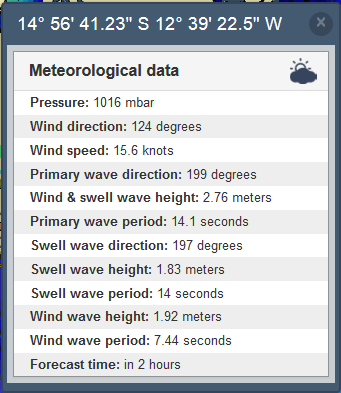
\includegraphics[width=0.35\textwidth]{img/weather_pufi}
            \end{center}
        \end{frame}

        % makes a node appear in TikZ mindmap, usage: `visible on=<n>`
        \tikzset{
            invisible/.style={opacity=0},
            visible on/.style={alt={#1{}{invisible}}},
            alt/.code args={<#1>#2#3}{%
                \alt<#1>{\pgfkeysalso{#2}}{\pgfkeysalso{#3}} % \pgfkeysalso doesn't change the path
            },
        }

        \begin{frame}{Why and API?}
            \begin{center}
                \begin{tikzpicture}[scale=1]
                    \path[mindmap,
                          concept,
                          text=white,
                          level 1/.append style={level distance=3cm},
                          every node/.append style={scale=0.6}]
                            node[concept] {Commercial API Service}
                            [clockwise from=0]
                            child[concept color=magenta!50]{node[concept]{Comms API}}
                            child[concept color=orange, visible on=<2->]{node[concept]{Weather API}}
                            child[concept color=green!50!black]{node[concept]{Event API}}
                            child[concept color=blue]{node[concept]{Corresp. API}}
                            child[concept color=red]{node[concept]{SIS API}};
                            \node[draw,align=left,visible on=<3->,style=rounded corners] at (3,2.5) {
                                \textit{modularity}, \textit{composition},\\\textit{separation, extensibility}\\
                                \tiny{\textit{Eric S. Raymonds, ``The Art of UNIX Programming'', 2003}}
                            };
                \end{tikzpicture}
            \end{center}
        \end{frame}

    \subsection{GRIB data}

        \begin{frame}{Show me a GRIB! \small{(1 layer)}}
            \begin{figure}
                \centering
                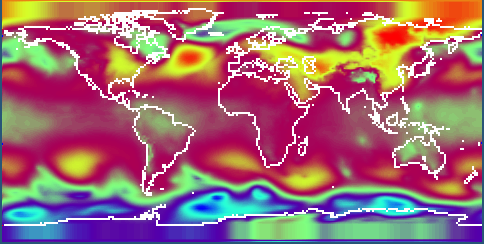
\includegraphics[width=0.8\textwidth]{img/nc_screen}
                \caption{Pressure Reduced at mean sea level, Tidetech data}
                \label{fig:prmsl}
                \scriptsize
                \begin{itemize}
                    \item GRIB: \textbf{G}eneral \textbf{R}egularly-distributed \textbf{I}nformation in \textbf{B}inary form
                    \item current data provider: Tidetech Pty Ltd, daily updates
                    \item avg file size: 9 Mb
                    \item timespan: 6 days
                \end{itemize}
            \end{figure}
        \end{frame}

        \begin{frame}{Something is rotten in the state of Denmark}
            \begin{columns}[c]
                \column{.4\textwidth}
                \onslide<1->{
                    \footnotesize{17 layers:}
                    \tiny
                    \begin{itemize}
                        \item \temporal<3>{latitudes array (-90, +90)}{\textbf{latitudes array (-90, +90)}}

                        \item \temporal<3>{longitudes array (-180, +180)}{\textbf{longitudes array (-180, +180)}}

                        \item minutes from first observation
                        \item string with datetime
                        \item initial\_time3\_hours (time)
                        \item PeakWaveDirection
                        \item SignificantWaveHeight
                        \item PressureReduced0SL
                        \item PeakWavePeriod
                        \item SwellWavesMeanPeriod
                        \item SwellWavesSignificantHeight
                        \item SwellWavesDirection
                        \item WindUComponent
                        \item WindVComponent
                        \item WindWavesMeanPeriod
                        \item WindWavesSignificantHeight
                    \end{itemize}
                }
                \column{.6\textwidth}
                \onslide<2->{
                    \scriptsize
                    \begin{itemize}
                        \item weather GRIB is actually a bundle of arrays
                        \item each record is independent
                        \item GRIB is not a database table: no indexes, \temporal<3>{no foreign keys}{\textbf{no foreign keys}}

                        \item as of PostGIS 1.5, there is no way to import GRIB data as raster (and query it)
                        \item each provider's GRIB structure is different (no common schema)\\\vspace{0.1\textheight}
                        \onslide<3>{\scriptsize{
                            No, you can't do this:\\\vspace{0.05\textheight}
                            \texttt{SELECT pressure\\FROM weather\\WHERE time=now, lat=41.5, lon=10}
                    }}
                    \end{itemize}
                }
            \end{columns}
        \end{frame}

    %\subsection{PurpleFinder}
    %
    %    \begin{frame}{Old approach: PurpleFinder}
    %    \end{frame}

    \subsection{NumPy}

        \begin{frame}{Current approach: NumPy NetCDF parsing}
            Long story short: if you can't query it, \textbf{parse} it.
            \pause
            \begin{description}
                \item[NetCDF]\textit{Network Common Data Form}, OGC format for sharing array-oriented data
            \end{description}
            \pause
            \begin{center}
                \resizebox{0.9\textwidth}{!}{%
                    \begin{tikzpicture}
                        \input{img/weather-scheme}
                    \end{tikzpicture}
                }
            \end{center}
            \vfill
            \pause
            \begin{itemize}
                \item conversion tool: \texttt{ncl} (NCAR Command Language)
                \item conversion time: nearly 1 sec
            \end{itemize}
        \end{frame}

        \begin{frame}{Inside the NetCDF}

            \texttt{pip install scipy}\\
            \texttt{from scipy.io import netcdf}\\
            \texttt{nc = netcdf.netcdf\_file('somefile', 'r')}
            \vfill
            \begin{equation*}
                $\text{weather}$ = 
                    \onslide<2->{
                        \tikz[baseline]{
                            \node[fill=blue!20,anchor=base] (t1)
                            {$\left[\text{layer}\right]$};
                        } +
                    }
                    \onslide<3->{
                        \tikz[baseline]{
                            \node[fill=red!20, ellipse,anchor=base] (t2)
                            {$\left[\text{time slot}\right]$};
                        } +
                    }
                    \onslide<4->{
                        \tikz[baseline]{
                            \node[fill=green!20,anchor=base] (t3)
                            {$\left[\text{lat}\right]$};
                        } +
                    }
                    \onslide<5->{
                        \tikz[baseline]{
                            \node[fill=green!20,anchor=base] (t4)
                            {$\left[\text{lon}\right]$};
                        }
                    }
            \end{equation*}
        \end{frame}

\section{Time: slots}

    \begin{frame}{Time specs}
        \begin{itemize}
            \item first forecast in each GRIB 6 am
            \pause
            \item each time slot has a 6 hours span
            \pause
            \item each GRIB files has a temporal span of 7 days
            \pause
            \item each GRIB contains $(6\text{h} \cdot 4) \cdot 7 = 168$ slots
        \end{itemize}
    \end{frame}

    \begin{frame}{Daily job: day 1}
        \begin{itemize}
            \item a new GRIB is downloaded from FTP; MD5sum compared with latest record
            \item NetCDF is generated and parsed
            \item all the timeslots are saved in a Django model (\texttt{Timeslot})
            \item API call: the requested date is fetched from the model
            \item the \texttt{Timeslot} has foreignkey to the actual NetCDF file
        \end{itemize}
        \vspace{0.05\textwidth}
        \startchronology[startyear=0,stopyear=84]
            \chronoperiode[dates=false,color=red]{6}{84}{}
            \chronograduation{24}
            \chronoevent[date=false]{6}{\tiny{6 am}}
            \chronoevent[date=false]{12}{\tiny{12 am}}
            \chronoevent[date=false]{18}{\tiny{6 pm}}
            \chronoevent[date=false]{30}{\tiny{6 am}}
        \stopchronology
    \end{frame}

    \begin{frame}{Daily job: day 2}
        \begin{itemize}
            \item a new GRIB is downloaded from FTP; MD5sum compared with latest record
            \item NetCDF is generated and parsed
            \item the \texttt{first} timeslot from the new grib is taken
            \item all timeslots with $\text{date}>=\text{first}$ are deleted
            \item all new timeslots are saved and will reference the new NetCDF
        \end{itemize}
        \vspace{0.05\textwidth}
        \startchronology[startyear=0,stopyear=84]
            \chronoperiode[dates=false]{6}{30}{}
            \chronoperiode[dates=false]{30}{84}{}
            \chronograduation{24}
            \chronoevent[date=false]{6}{\tiny{6 am}}
            \chronoevent[date=false]{12}{\tiny{12 am}}
            \chronoevent[date=false]{18}{\tiny{6 pm}}
            \chronoevent[date=false]{30}{\tiny{6 am}}
            \chronoevent[date=false]{36}{\tiny{12 am}}
            \chronoevent[date=false]{42}{\tiny{6 pm}}
        \stopchronology
    \end{frame}

    % TODO: find the nearest slot

\section{Space: grid}

    \begin{frame}{Messing with the coordinates}
        \begin{itemize}
            \item spatial grid unit in GRIB files: no standard
                \begin{itemize}
                    \item item grid size loaded from Django settings (adjustable)
                \end{itemize}
            \item Tidetech: grid of cells with side of 1.5 degrees
                \begin{itemize}
                    \item $\text{longitudes} = 360/1.5 = 240 x$
                    \item $\text{latitudes} = 180/1.5 = 121 y$
                \end{itemize}
        \end{itemize}
        \pause
        Find the correct array:
        \begin{enumerate}
            \item convert lat/lon values ($x={-180,+180}$, $y={-90,+90}$) on a matrix with size ($x={0,240}$, $y={0,121}$)
            \pause
            \item round searched point to the nearest point on the grid
            \pause
            \item parse the NetCDF to find the array matching that point
            \pause
            \item iterate on all layers to get complete forecast
            \pause
            \item booooring
        \end{enumerate}
    \end{frame}

    \begin{frame}{Example}
        \begin{block}{Homework}
            Get weather for $\text{lon}=15$, $\text{lat}=30$.
        \end{block}
        \vspace{0.05\textheight}
        Get the index of the cells on a matrix of $x={0,240}$, $y={0,121}$:
        \begin{center}
            \texttt{lat\_idx = convert\_latitude(lat) = 20}\\
            \texttt{lon\_idx = convert\_longitude(lon) = 130}
        \end{center}
        Round the indexes to the nearest cell in the matrix:
        \begin{center}
            \texttt{round\_to\_grid(lat\_idx, lon\_idx) = 19.5, 130}
        \end{center}
    \end{frame}

    \begin{frame}{Example}
        Finally, get weather parsing the array with the correct indexes:
        \vspace{0.05\textheight}
        \scriptsize{
            \texttt{from weatherapi.utils import TimeSlot}\\
            \texttt{slot = get\_nearest\_slot(datetime)}\\
            \texttt{layer\_data = slot.grib.get\_layer\_content(layers)}\\
            \texttt{for name in layer\_data.keys():}\\
            \texttt{~~~~value = layer\_data.get(name)[slot\_n][latitude][longitude]}\\
        }
        \vspace{0.05\textheight}
        In the response, append metadata with the actual location of the forecast:
        \texttt{get\_coord\_from\_grid(130, 19.5) = 15.75, 29.25}
    \end{frame}

\section{Response structure}

\begin{frame}{Try it}
        \begin{center}
            \large https://weatherapi-test.polestar-internal.com/api/doc\\
            \vspace{0.05\textheight}
            d9f7b8249ba56c91d7edadea074454d8884e0190\\
            admin
        \end{center}
    \end{frame}

\section{Future}

    \begin{frame}{Nice to have}
        \begin{description}
            \item[PostGIS 2: raster2pgsql GRIB support]~\\
                    \texttt{gdalwarp -t\_srs EPSG:4326 somefile.grib somefile-epsg-4326.grib}\\
                    \texttt{raster2pgsql -M -a somefile-epsg-4326.grib somefile.sql}

            \item[forecast caching]~\\cache the forecast for the current day
            \item[get forecast along track]~\\extract forecast for a future period along a list of positions
        \end{description}
    \end{frame}

\section{Thanks}

    \begin{frame}{Random gratitude}
        \vspace{0.05\textheight}
        For helpful suggestions, pointings, etc.
        \begin{itemize}
            \item Phelps
            \item Corps
            \item Bretschneider
            \item Devops
        \end{itemize}
    \end{frame}

\section{Questions?}

\begin{frame}{Questions?}
        \begin{center}
            \Huge{?}
        \end{center}
    \end{frame}

\section{Who's next}

    \begin{frame}{Questions}
        \begin{center}
            \Huge{In der nächsten Folge:}\\\onslide<2->{Marcel}
        \end{center}
    \end{frame}

\end{document}
